\section{概率代理}
\label{sec:bo-surrogate}

怎样用一个读数更新没有被评价的位置的认识？这要求模型做到两件事，一是对每个候选点给出可能函数值的分布，二是说清不同位置之间怎样关联，否则一个位置的读数对其他位置不起作用。满足这两点、用来代替昂贵目标接受查询的模型，称为\term{概率代理}（probabilistic surrogate）。

本节以高斯过程为主说明这个接口。贝叶斯优化并不依赖高斯过程，只要模型能给出相应的预测分布，例如贝叶斯神经网络、树模型的集成，也可以代入后面的选点规则，只是计算的具体公式不同。

\subsection{高斯过程先验}
\label{sec:bo-gp-prior}

先看模型要表达的直觉：相近的参数，通常给出相近的仿真结果。这句话有两层意思。其一，单看一个位置，函数值可能的范围是一个分布。其二，两个位置离得越近，它们的函数值越同涨同落。用协方差描述第二层意思最直接，而最便于计算的联合分布是多元高斯分布。

\begin{definition}[高斯过程]
\label{def:bo-gp}
设$m_0:\bm{C}\to\mathbb{R}$，$k:\bm{C}\times\bm{C}\to\mathbb{R}$。若对任意有限个点$\bm{x}_1,\ldots,\bm{x}_n\in\bm{C}$，向量$(F(\bm{x}_1),\ldots,F(\bm{x}_n))^\top$都服从多元高斯分布，且
\begin{equation}
 \mathbb{E}[F(\bm{x})]=m_0(\bm{x}),\qquad
 \operatorname{Cov}(F(\bm{x}),F(\bm{x}'))=k(\bm{x},\bm{x}'),
 \label{eq:bo-gp}
\end{equation}
就称随机函数$F$是以$m_0$为\term{均值函数}（mean function）、以$k$为\term{协方差核}（covariance kernel）的\term{高斯过程}（Gaussian process，GP）。
\end{definition}

定义只谈有限个点，这正是它好用的地方。一次计算只会碰到有限个位置，手头需要的总是一个普通的多元高斯分布。

核$k$不能随便写。把几个位置的函数值作线性组合，方差必须非负。对任意实数$a_1,\ldots,a_n$，
\[
 0\leq\operatorname{Var}\Bigl(\sum_{i=1}^n a_iF(\bm{x}_i)\Bigr)
 =\sum_{i=1}^n\sum_{j=1}^n a_ia_jk(\bm{x}_i,\bm{x}_j)
 =\bm{a}^\top\bm{K}\bm{a},
\]
其中$\bm{K}$是元素为$k(\bm{x}_i,\bm{x}_j)$的矩阵。所以$k$必须对称，且任意有限组点上的$\bm{K}$都半正定。反过来，满足这两条的$k$配上任意均值函数，确实对应一个高斯过程，证明要用到有限维分布族的相容性与延拓定理，这里只使用结论。

\paragraph{贯穿例的核}
本章取$m_0\equiv0$，并取
\begin{equation}
 k(x,x')=2^{-(x-x')^2}.
 \label{eq:bo-example-kernel}
\end{equation}
它是常用的\term{平方指数核}（squared exponential kernel）$\exp(-(x-x')^2/(2\ell^2))$在$\ell^2=1/(2\ln2)$时的情形，$\ell\approx0.85$。选这个数只是为了手算：间距$1,2,3$的相关系数分别是$1/2,1/16,1/512$。先验方差$k(x,x)=1$表示模型认为函数值大致在$\pm2$内，这与表~\ref{tab:bo-readings}的数量级相符。

取三个相邻位置$x=3,4,5$，核矩阵为
\[
 \bm{K}=\begin{bmatrix}1&1/2&1/16\\1/2&1&1/2\\1/16&1/2&1\end{bmatrix}.
\]
三个顺序主子式依次为
\[
 1,\qquad \frac34,\qquad \frac{135}{256},
\]
全部为正，所以这个$\bm{K}$正定。

\paragraph{核规定了模型愿意相信的变化尺度}
参数$\ell$称为\term{长度尺度}（length scale），它回答“隔多远的两个点就基本无关了”。图~\ref{fig:bo-kernel-scales}比较了三个取值。$\ell$小时相关性衰减快，先验样本频繁起伏；$\ell$大时样本缓慢变化。三条样本用的是同一组随机数，差别完全来自核。

\begin{BookInlineFigure}
 \centering
 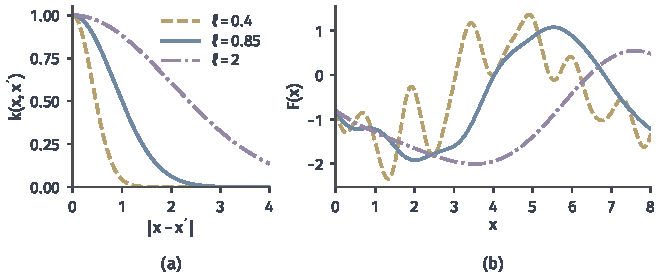
\includegraphics[width=112mm]{figures/05-optimization/05-stochastic-optimization/matplotlib/bo-kernel-scales/figure.pdf}
 \caption{长度尺度的作用。(a)平方指数核随距离的衰减，$\ell=0.85$是贯穿例的取值。(b)用同一组标准正态随机数生成的三条先验样本，线型与(a)对应。长度尺度越大，样本越缓慢。}
 \label{fig:bo-kernel-scales}
\end{BookInlineFigure}

所以核不只是计算工具，它是我们事先下的一个赌注。选了$\ell$，就等于声明目标不会比这个尺度变化得更快。这一声明可能错，第~\ref{sec:bo-model-specification}节专门讨论错了会怎样。

\subsection{后验预测}
\label{sec:bo-posterior}

先用两个位置看清更新是怎么发生的。考虑$x=3$和$x=4$，由式~\eqref{eq:bo-example-kernel}，
\[
 \begin{bmatrix}F(3)\\F(4)\end{bmatrix}
 \sim N\left(\begin{bmatrix}0\\0\end{bmatrix},
 \begin{bmatrix}1&1/2\\1/2&1\end{bmatrix}\right).
\]
现在只评价$x=3$，无噪声地读到$F(3)=1$。关键是把$F(4)$拆成“能由$F(3)$解释的部分”和“剩余部分”：
\[
 F(4)=\tfrac12F(3)+R.
\]

系数$1/2$的选法是让$R$与$F(3)$不相关：
\[
 \operatorname{Cov}(R,F(3))=\tfrac12-\tfrac12\cdot1=0.
\]
联合高斯时不相关就意味着独立，所以读到$F(3)$不改变$R$的分布。$R$的方差为
\[
 \operatorname{Var}(R)=1-2\cdot\tfrac12\cdot\tfrac12+\tfrac14\cdot1=\tfrac34.
\]
代入$F(3)=1$，得到
\[
 F(4)\mid F(3)=1\ \sim\ N\bigl(\tfrac12,\tfrac34\bigr).
\]

虽然没有评价$x=4$，这里的均值从$0$变成了$0.5$，方差从$1$降到了$0.75$。图~\ref{fig:bo-conditional-slice}中，(a)的椭圆是联合分布的等高线，在$F(3)=1$处竖切一刀，得到(b)中的绿线。椭圆是斜的，切线才偏离中心；若相关系数为$0$，椭圆不倾斜，切出来的分布就和先验一样，读数不传递任何信息。

\begin{BookInlineFigure}
 \centering
 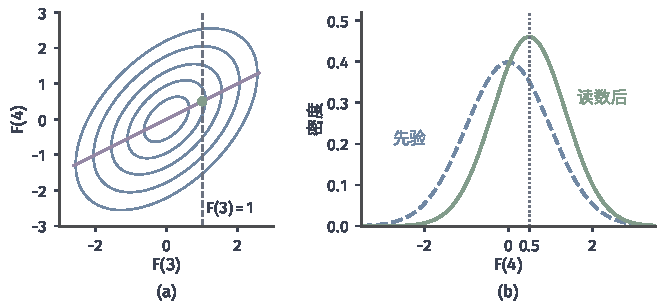
\includegraphics[width=112mm]{figures/05-optimization/05-stochastic-optimization/matplotlib/bo-conditional-slice/figure.pdf}
 \caption{读数怎样传到相关的位置。(a)蓝色椭圆是$(F(3),F(4))$的联合分布等高线，相关系数$1/2$，紫线是条件均值$F(4)=F(3)/2$，竖虚线是读数$F(3)=1$，绿点是该读数下$F(4)$的条件均值。(b)蓝虚线是$F(4)$的先验$N(0,1)$，绿线是读数后的$N(1/2,3/4)$。}
 \label{fig:bo-conditional-slice}
\end{BookInlineFigure}

一般情形只是把这种拆分写成矩阵。记$\bm{K}_t$为$t\times t$矩阵，元素是$k(\bm{x}_i,\bm{x}_j)$；$\bm{k}_t(\bm{x})$是长度$t$的向量，第$i$个分量是$k(\bm{x},\bm{x}_i)$；$\bm{y}_t$是读数向量；$\bm{m}_{0,t}$是先验均值在各评价点处的取值。读数可能含噪，设$y_i=F(\bm{x}_i)+\varepsilon_i$，$\varepsilon_i\sim N(0,\tau^2)$，彼此独立，且与$F$独立；$\tau=0$表示无噪声。

\begin{theorem}[高斯过程的后验]
\label{thm:bo-posterior}
设$F$是高斯过程，评价点固定，核与噪声参数已知，$\bm{A}_t=\bm{K}_t+\tau^2\bm{I}$可逆。则给定$\bm{y}_t$，$F$仍是高斯过程，其后验均值与后验协方差为
\begin{align}
 m_t(\bm{x})&=m_0(\bm{x})+\bm{k}_t(\bm{x})^\top\bm{A}_t^{-1}(\bm{y}_t-\bm{m}_{0,t}),
 \label{eq:bo-post-mean}\\
 c_t(\bm{x},\bm{x}')&=k(\bm{x},\bm{x}')-\bm{k}_t(\bm{x})^\top\bm{A}_t^{-1}\bm{k}_t(\bm{x}').
 \label{eq:bo-post-cov}
\end{align}
特别地，记$s_t^2(\bm{x})=c_t(\bm{x},\bm{x})$，则
\begin{equation}
 F(\bm{x})\mid\mathcal{D}_t\sim N\bigl(m_t(\bm{x}),s_t^2(\bm{x})\bigr).
 \label{eq:bo-post-marginal}
\end{equation}
\end{theorem}

\begin{proof}
取任意有限组候选点，$F$在这些点与读数向量合起来是联合高斯的。对一个候选点$\bm{x}$，令
\[
 \bm{a}=\bm{A}_t^{-1}\bm{k}_t(\bm{x}).
\]
定义剩余量
\[
 R(\bm{x})=F(\bm{x})-m_0(\bm{x})-\bm{a}^\top(\bm{y}_t-\bm{m}_{0,t}),
\]
这里$\bm{y}_t$理解为随机向量。

读数的协方差矩阵是$\bm{A}_t$，$F(\bm{x})$与读数的协方差向量是$\bm{k}_t(\bm{x})$，于是
\[
 \operatorname{Cov}(R(\bm{x}),\bm{y}_t)=\bm{k}_t(\bm{x})-\bm{A}_t\bm{a}=\bm{0}.
\]
联合高斯下，不相关推出独立，所以$\mathcal{D}_t$不改变$R(\bm{x})$的分布，它的均值仍是$0$。把读数的实际值代入$F(\bm{x})$的分解式，条件均值就是式~\eqref{eq:bo-post-mean}。

设$R'$是$\bm{x}'$处对应的剩余量，$\bm{a}'=\bm{A}_t^{-1}\bm{k}_t(\bm{x}')$。给定读数后$F(\bm{x})$与$F(\bm{x}')$的随机部分只有$R$与$R'$，因此
\[
 \begin{aligned}
 \operatorname{Cov}(R,R')
 &=k(\bm{x},\bm{x}')-\bm{a}^\top\bm{k}_t(\bm{x}')-\bm{a}'^\top\bm{k}_t(\bm{x})+\bm{a}^\top\bm{A}_t\bm{a}'\\
 &=k(\bm{x},\bm{x}')-\bm{k}_t(\bm{x})^\top\bm{A}_t^{-1}\bm{k}_t(\bm{x}').
 \end{aligned}
\]
这就是式~\eqref{eq:bo-post-cov}。任意有限组点上同样成立，所以后验仍是高斯过程。
\end{proof}

这个证明用到联合高斯下不相关推出独立，条件高斯的一般公式及其矩阵推导可参考\BookChapterRef{chap:random-vectors}{卷七第6章“随机向量”}；把核视为函数上的先验来做回归的一般理论，可参考\BookChapterRef{chap:nonparametric-inference}{卷八第2章“非参数分布与函数推断”}。

读这两个公式时，注意三件事。第一，后验方差~\eqref{eq:bo-post-cov}不含读数$\bm{y}_t$，只取决于评价放在哪里，好读数和坏读数减少的不确定性相同。第二，无噪声时$m_t(\bm{x}_i)=y_i$，$s_t(\bm{x}_i)=0$，模型穿过读数。第三，$c_t(\bm{x},\bm{x}')$要保留，不能只留方差，后面联合抽样和批量选点都要用到不同候选点之间的后验协方差。

定理假设评价点固定，而实际的$\bm{x}_{t+1}$依赖之前的读数。公式仍然成立，原因是选点规则只看$\mathcal{D}_t$：写出整条数据的似然时，选点这一步给出的因子不依赖$F$，它在归一化时被消去，后验仍只由读数的高斯因子决定。条件分布的一般含义可参考\BookChapterRef{chap:conditional-expectation}{卷七第10章“条件期望”}。

\paragraph{贯穿例：三个读数后的后验}
评价$x=1,4,7$，读数$\bm{y}_3=(0.2,0.7,-0.3)^\top$。核矩阵是
\[
 \bm{K}_3=\begin{bmatrix}1&2^{-9}&2^{-36}\\2^{-9}&1&2^{-9}\\2^{-36}&2^{-9}&1\end{bmatrix},
\]
其中$2^{-9}\approx0.002$。解线性方程$\bm{K}_3\bm{w}=\bm{y}_3$，得到
\[
 \bm{w}=\bm{K}_3^{-1}\bm{y}_3\approx(0.1986,\ 0.7002,\ -0.3014)^\top.
\]

看未评价的$x=6$。到三个评价点的距离是$5,2,1$，所以
\[
 \bm{k}_3(6)=(2^{-25},\ 1/16,\ 1/2)^\top.
\]
由式~\eqref{eq:bo-post-mean}，
\[
 m_3(6)=\bm{k}_3(6)^\top\bm{w}\approx0.0625\times0.7002-0.5\times0.3014\approx-0.107.
\]
由式~\eqref{eq:bo-post-cov}，
\[
 s_3^2(6)=1-\bm{k}_3(6)^\top\bm{K}_3^{-1}\bm{k}_3(6)\approx0.746,
\]
即$s_3(6)\approx0.864$。把$2^{-9}$按$0$手算，会得到$-0.106$和$0.746$，差别只在第三位小数。

图~\ref{fig:bo-posterior-sequence}是读数逐个加入时的后验。第一个读数只影响$x=1$附近，其他地方后验几乎还是先验。后面的读数逐段收紧不确定带。深色的后验均值并没有“找到”$x=6$的谷，这很自然：三个点都不在谷里，模型没有理由想象到它。正是这种“均值还不低、但不确定带向下伸得很远”的区域，需要由下一节的规则来评估。

\begin{BookInlineFigure}
 \centering
 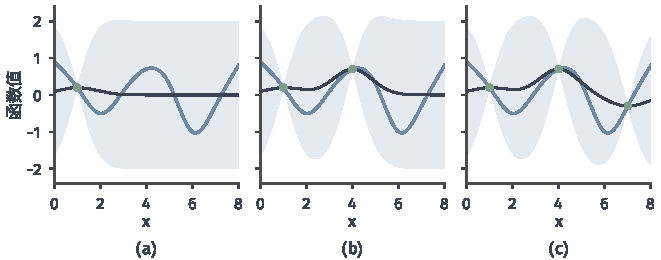
\includegraphics[width=112mm]{figures/05-optimization/05-stochastic-optimization/matplotlib/bo-posterior-sequence/figure.pdf}
 \caption{后验随读数更新。蓝线是目标$f$，深色线是后验均值$m_t$，浅蓝带是$m_t\pm2s_t$，绿点是读数。(a)只有$x=1$；(b)加入$x=4$；(c)加入$x=7$。}
 \label{fig:bo-posterior-sequence}
\end{BookInlineFigure}

计算量也要记一笔。对$\bm{A}_t$作一次Cholesky分解约需$t^3/3$次运算，见\BookChapterRef{chap:direct-linear-solvers}{卷二第12章“线性方程的直接求解”}；此后每个候选点的均值需$O(t)$次运算，方差需$O(t^2)$次。贝叶斯优化中$t$通常只有几十到几百，这笔开销相对一次昂贵评价可以忽略，第~\ref{sec:bo-budget}节再核算它什么时候不能忽略。

\subsection{模型设定}
\label{sec:bo-model-specification}

上面都假定核与噪声参数已知。实际问题中$\ell$、先验方差等\term{超参数}（hyperparameter）并不知道，这就有了本节的问题：模型的这些设定错了会怎样，又该如何对待它们的不确定性。

\paragraph{边缘似然与直接代入}
常用办法是看哪组超参数最能解释已有读数。把超参数记为$\bm{\theta}$，读数的边缘分布是$N(\bm{m}_{0,t},\bm{A}_t(\bm{\theta}))$，其对数密度
\begin{equation}
 \log p(\bm{y}_t\mid\bm{\theta})=-\tfrac12\bm{r}^\top\bm{A}_t^{-1}\bm{r}-\tfrac12\log\det\bm{A}_t-\tfrac t2\log(2\pi)
 \label{eq:bo-marginal-likelihood}
\end{equation}
称为\term{边缘似然}（marginal likelihood）的对数，其中$\bm{r}=\bm{y}_t-\bm{m}_{0,t}$。第一项奖励拟合读数，第二项惩罚过于灵活的模型。常见做法是取使它最大的$\widehat{\bm{\theta}}$，然后把它当作真值代入定理~\ref{thm:bo-posterior}。

直接代入回避了一个事实：超参数本身也拿不准。把不确定性计入的做法是对超参数的后验分布积分，得到混合预测。若$\bm{\theta}$只有有限个候选，后验概率为$w_j$，候选$j$给出的均值和方差为$m^{(j)},v^{(j)}$，则由全方差公式，
\begin{equation}
 \begin{gathered}
 \bar m=\sum_jw_jm^{(j)},\\
 \bar v=\sum_jw_jv^{(j)}+\sum_jw_j\bigl(m^{(j)}-\bar m\bigr)^2.
 \end{gathered}
 \label{eq:bo-mixture}
\end{equation}
第一项是平均的方差，第二项是不同超参数之间的分歧。第二项非负，所以混合预测的方差不小于各候选方差的加权平均，分歧越大增加越多。

\paragraph{例：两个候选长度尺度}
仍用三个读数，比较$\ell\approx0.85$和$\ell=3$，两者的先验概率相等。由式~\eqref{eq:bo-marginal-likelihood}算得对数边缘似然分别约为$-3.067$和$-3.106$，几乎相同，按贝叶斯公式得到后验概率
\[
 w_1\approx0.51,\qquad w_2\approx0.49.
\]
三个读数不足以区分这两种解释。

两种解释在$x=6$处的预测却差得很远：
\[
 \begin{aligned}
 \ell\approx0.85:&\quad m=-0.107,\quad v=0.746,\\
 \ell=3:&\quad m=0.093,\quad v=0.015.
 \end{aligned}
\]
由式~\eqref{eq:bo-mixture}，混合预测的均值和方差为
\[
 \bar m\approx-0.009,\qquad \bar v\approx0.398.
\]

若只取$\ell=3$直接代入，方差$0.015$比混合预测小了约$26$倍。图~\ref{fig:bo-model-specification}(b)显示，长度尺度大的模型在$x=6$处把标准差算得很小，而真实值$-1.0$远在它的不确定带之外。这正是直接代入的风险：边缘似然选中了一个看上去同样好的解释，却丢掉了“还有另一种解释”这条信息。

\begin{BookInlineFigure}
 \centering
 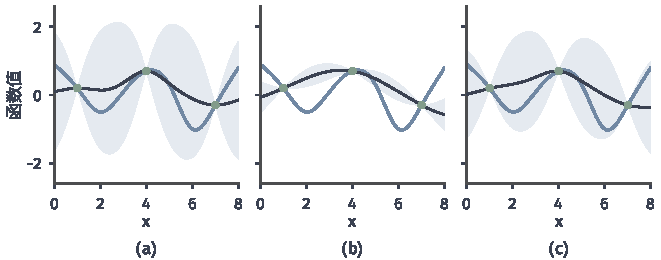
\includegraphics[width=112mm]{figures/05-optimization/05-stochastic-optimization/matplotlib/bo-model-specification/figure.pdf}
 \caption{同样三个读数下的不同模型设定。蓝线是目标，深色线是预测均值，浅蓝带是均值上下两倍标准差。(a)$\ell\approx0.85$；(b)$\ell=3$，不确定带很窄，却没有盖住$x=6$附近的谷；(c)两者按边缘似然加权的混合预测，读数之间的方差反映了两种解释的分歧。}
 \label{fig:bo-model-specification}
\end{BookInlineFigure}

\paragraph{设定要回到问题来检查}
长度尺度隐含一个假设：同样的距离代表同样的变化幅度。输入的尺度是否合适直接关系这个假设。例如学习率类的参数从$10^{-4}$变到$1$，在原始坐标上$10^{-4}$与$10^{-3}$几乎重合，但它们的效果可能相差很多；改用$\log_{10}$坐标后，相邻量级的距离才都等于$1$。多维问题中各坐标的单位不同，通常给每个坐标各设一个长度尺度。

先验的光滑程度也要与问题相符。平方指数核的样本无穷次可微，目标若有折点或跳跃，模型会用过短的长度尺度去迁就，导致全局方差偏大。可微性有限的核，如Mat\'ern族，常用来表达较弱的光滑假设。

读数本身可以检验模型。依次去掉第$i$个读数，用其余读数预测它，得到留一标准化残差
\begin{equation}
 e_i=\frac{y_i-m_{-i}(\bm{x}_i)}{\sqrt{s_{-i}^2(\bm{x}_i)+\tau^2}}.
 \label{eq:bo-loo}
\end{equation}
模型合适时这些数大致像标准正态的取值，大量绝对值超过$3$说明模型与读数不符。贯穿例的三个读数相距较远，其余读数几乎不影响被去掉的位置，$e_i$约等于读数本身，$0.2,0.7,-0.3$都不大。可是读数太少时这个检查的力量也很弱，通过检查不等于模型正确。

低方差只说明“在这个模型下”不确定性小，不能直接等同于目标已经被准确掌握。图~\ref{fig:bo-model-specification}(b)是一个具体的反例。后面几节的后验都默认超参数固定，这是为了把选点逻辑讲清楚；实际使用时，每轮通常重新估计或积分超参数，第~\ref{sec:bo-noise-variances}节还会看到这样做对方差的影响。
